\documentclass{article}
\usepackage{listings} % For code formatting
\usepackage[utf8]{inputenc}  % For encoding support
\usepackage{amsmath}         % For mathematical formatting
\usepackage{graphicx}        % For including images
\usepackage{xcolor}
\usepackage[a4paper, left=0.5in, right=0.5in, top=0.5in, bottom=0.5in]{geometry}  % Adjust margins here
\usepackage{tcolorbox}
\usepackage{inconsolata}  % Use Inconsolata font (or replace with your choice)

% Define colors
\definecolor{codebg}{RGB}{240, 240, 240}  % Light gray background
\definecolor{framecolor}{RGB}{100, 100, 100}  % Dark gray frame
\definecolor{titlebg}{RGB}{30, 30, 30}  % Dark title background
\definecolor{titlefg}{RGB}{255, 255, 255}  % White title text

% Custom lstset
\lstset{
    language=C++,                    
    basicstyle=\ttfamily\footnotesize\fontfamily{zi4}\selectfont, % Use Inconsolata
    keywordstyle=\bfseries\color{blue},        
    commentstyle=\itshape\color{gray},        
    stringstyle=\color{red},          
    numbers=left,                     
    numberstyle=\tiny\color{blue},    
    frame=single,                     
    breaklines=true,                   
    captionpos=b,                      
    backgroundcolor=\color{codebg},  % Light gray background
    rulecolor=\color{framecolor},    % Dark frame
    tabsize=4                         
}

% Custom command to add a styled heading
\newtcbox{\codebox}{colback=titlebg, colframe=titlebg, colupper=titlefg, 
  boxrule=0pt, arc=5pt, left=5pt, right=5pt, top=3pt, bottom=3pt}

\title{Parallel Programming Assignment 1}
\author{Ayush Raina, 22148}
\date{\today}

\begin{document}

\maketitle

\section*{Merge Sort}
Merge Sort is a divide and conquer algorithm that divides the input array into two halves, recursively sorts the two halves, and then merges the sorted halves. The time complexity of Sequential Merge Sort is $\mathcal{O}(n \log n)$. We will implement some parallel versions of Merge Sort using CUDA C++ and Open MP. 

\subsection*{Benchmarking}
We will use array size $\sim 16.7$ million for initial observations. Later we will report observations with different array Sizes. Sequential Algorithm took $\sim 4615$ ms = $4.615$ sec to sort this array of size $16.7$ million. We will use this as a reference to calculate speedup.

\subsection*{Merge Sort Version 1}
In this version, we will assume that division of array is done into single elements. We will start merging sorted sub lists of size $1,2,4,8,..$ and so on sequentially in parallel. Assume our array is denoted by $\mathcal{A}$

\begin{itemize}
  \item In Iteration 1, we will merge $(\mathcal{A}[0], \mathcal{A}[1])$, $(\mathcal{A}[2], \mathcal{A}[3])$, $(\mathcal{A}[4], \mathcal{A}[5])$, $(\mathcal{A}[6], \mathcal{A}[7])$ and so on.
  \item In Iteration 2, we will merge $(\mathcal{A}[0-1], \mathcal{A}[2-3])$, $(\mathcal{A}[4-5], \mathcal{A}[6-7])$ and so on.
  \item In Iteration 3, we will merge $(\mathcal{A}[0-3], \mathcal{A}[4-7])$ and so on.
\end{itemize}

\codebox{Implementation 1}

\begin{lstlisting}
  __global__ void ParallelMergeKernel(int* input, int* output, int size, int window_size) {

    int tid = blockDim.x * blockIdx.x + threadIdx.x;
    if(tid >= size) return;

    // Calculate required indices for sublists
    int start_one = tid * window_size * 2;
    int end_one = min(start_one + window_size, size);

    int start_two = end_one;
    int end_two = min(start_two + window_size, size);

    // Sequential Merging of two sublists
    int i = start_one, j = start_two, k = start_one;

    while(i < end_one and j < end_two) {
        if(input[i] < input[j]) {
            output[k++] = input[i++];
        } else {
            output[k++] = input[j++];
        }
    }

    // Copy remaining elements in both cases
    while(i < end_one) {
        output[k++] = input[i++];
    }

    while(j < end_two) {
        output[k++] = input[j++];
    }
}
\end{lstlisting}

\subsection*{Analysis of Version 1}
In this version,we do not need $N$ threads in total, we need:
\begin{itemize}
  \item $\boxed{\text{threadsPerBlock} = {\frac{N + 2*\text{window\_size} - 1}{2*\text{window\_size}}}}$
  \item $\boxed{\text{blocksPerGrid} = \frac{N + \text{ threadsPerBlock - 1}}{\text{threadsPerBlock}}}$
\end{itemize}

Here are the execution times for different blockSizes and windowSizes:

\begin{center}
  \begin{tabular}{|c|c|c|}
    \hline
    \textbf{blockSize} & \textbf{Execution Time (ms)} & \textbf{Speedup} \\
    \hline

    16 & 2046 & 2.2556 \\
    32 & 2048 & 2.2534 \\
    64 & 2049 & 2.2523 \\
    128 & 2047 & 2.2545 \\
    256 & 2050 & 2.2512 \\
    
    \hline
  \end{tabular}
\end{center}

\subsection*{Optimization 1: Binary Search Based Merging}
In this version, we will use binary search to find the correct position of elements from one sublist in another sublist. Suppose $pos = k$, then first copy $k-1$ elements from first sublist to output array and then copy $k$ elements from second sublist to output array and continue.

\codebox{Implementation 2}

\begin{lstlisting}
__global__ void ParallelMergeKernel(int* input, int* output, int size, int window_size) {
    int tid = blockDim.x * blockIdx.x + threadIdx.x;
    if(tid >= size) return;

    // Calculate required indices for sublists
    int start_one = (tid * 2) * window_size;
    int end_one = min(start_one + window_size, size);

    int start_two = end_one;
    int end_two = min(start_two + window_size, size);

    if(start_one >= size) return;

    // Initialize pointers for output
    int i = start_one;
    int j = start_two;
    int k = start_one;

    // Binary search based merge
    while(i < end_one && j < end_two) {

        // Find position of input[j] in first subarray
        if(i < end_one) {
            int low = i, high = end_one, position = i;
            
            while(low < high) {
                
                int mid = low + (high - low) / 2;
                if(input[mid] <= input[j]) {
                    low = mid + 1;
                    position = low;
                } else {
                    high = mid;
                }
                
            }
            
            // Copy elements from first subarray up to the found position
            while(i < position) {
                output[k++] = input[i++];
            }
            
            // Copy element from second subarray
            output[k++] = input[j++];
        }
    }

    // Copy remaining elements from first subarray
    while(i < end_one) {
        output[k++] = input[i++];
    }

    // Copy remaining elements from second subarray
    while(j < end_two) {
        output[k++] = input[j++];
    }
}
\end{lstlisting}

\subsection*{Analysis of Optimization 1}
Here are the execution times for different blockSizes and windowSizes:

\begin{center}
  \begin{tabular}{|c|c|c|}
    \hline
    \textbf{blockSize} & \textbf{Execution Time (ms)} & \textbf{Speedup} \\
    \hline

    16 & 1541 & 2.9948 \\
    32 & 1540 & 2.9967 \\
    64 & 1544 & 2.9889 \\
    128 & 1549 & 2.9793 \\
    256 & 1543 & 2.9909 \\
    
    \hline
  \end{tabular}
\end{center}

\subsection*{Merge Sort in Open MP}
Here is the merge function which is mostly similar to sequential version:
\codebox{Implementation}

\begin{lstlisting}
void merge(vector<int>& arr, int left, int mid, int right) {
    vector<int> temp(right - left + 1);
    int i = left, j = mid + 1, k = 0;
    
    while (i <= mid and j <= right) {
        if (arr[i] <= arr[j])
            temp[k++] = arr[i++];
        else
            temp[k++] = arr[j++];
    }
    
    while (i <= mid) {
        temp[k++] = arr[i++];
    }

    while (j <= right) {
        temp[k++] = arr[j++];
    }

    for (i = 0; i < k; i++) {
        arr[left + i] = temp[i];
    }
    
}
\end{lstlisting}

\begin{lstlisting}
// Recursive merge sort function with OpenMP parallelization
// omp_set_num_threads = 24 is set in main function

void mergeSortParallel(vector<int>& arr, int left, int right, int depth = 0) {
    if (left < right) {
        int mid = left + (right - left) / 2;
        
        // Parallelize only up to a certain depth to avoid overhead
        if (depth < 4) {
            #pragma omp parallel sections
            {
                #pragma omp section
                mergeSortParallel(arr, left, mid, depth + 1);
                
                #pragma omp section
                mergeSortParallel(arr, mid + 1, right, depth + 1);
            }
        } else {
            mergeSortParallel(arr, left, mid, depth + 1);
            mergeSortParallel(arr, mid + 1, right, depth + 1);
        }
        
        merge(arr, left, mid, right);
    }
}
\end{lstlisting}

\subsection*{Analysis of Open MP Version}
Here are the execution time for Open MP  vs Sequential Merge Sort:

\begin{center}
  \begin{tabular}{|c|c|c|}
    \hline
    \textbf{Array Size} & \textbf{Execution Time (ms)} & \textbf{Speedup} \\
    \hline

    16.7 million & 2481 & 1.8657 \\
    
    \hline
  \end{tabular}
\end{center}

\subsection*{Experimenting with Different Array Sizes with CUDA}
Here are the execution times for different array sizes:

\begin{center}
  \begin{tabular}{|c|c|c|c|c|c|}
    \hline
    \textbf{Array Size} & \textbf{Sequential (ms)} & \textbf{CUDA (ms)} & \textbf{Speedup (CUDA v1)} & \textbf{CUDA v2} & \textbf{Speedup (CUDA v2)}\\
    \hline

    0.26 million & 60 & 37 & 1.62 & 28 & 2.14 \\
    0.52 million & 122 & 62 & 1.96 & 51 & 2.39 \\ 
    1.04 million & 252 & 204 & 1.23 & 96 & 2,625 \\
    2.09 million & 501 & 251 & 1.99 & 188 & 2.64 \\
    4.19 million & 1014 & 510 & 1.98 & 384 & 1.8657 \\
    8.39 million & 2085 & 1004 & 2.07 & 758 & 2.656 \\
    16.7 million & 4290 & 2075 & 2.06 & 1562 & 2.746 \\
    33.5 million & 8671 & 4061 & 2.13 & 3064 & 2.829 \\
    67.1 million & 17754 & 8208 & 2.16 & 6165 & 2.879 \\
    134.2 million & 36779 & 16040 & 2.292 & 12128 & 3.032 \\
    268.4 million & 75431 & 32747 & 2.303 & 24584 & 3.068 \\
    
    \hline
  \end{tabular}
\end{center}

\subsection*{Experimenting with Different Array Sizes with Open MP}

Here are the execution times for different array sizes:

\begin{center}
  \begin{tabular}{|c|c|c|}
    \hline
    \textbf{Array Size} & \textbf{Execution Time (ms)} & \textbf{Speedup} \\
    \hline

    0.26 million & 31 & 1.93 \\
    0.52 million & 65 & 1.87 \\
    1.04 million & 137 & 1.83 \\
    2.09 million & 278 & 1.80 \\
    4.19 million & 572 & 1.77 \\
    8.39 million & 1182 & 1.76 \\
    16.7 million & 2437 & 1.76 \\
    33.5 million & 5081 & 1.70 \\
    67.1 million & 10373 & 1.71 \\
    134.2 million & 21479 & 1.71 \\
    268.4 million & 44450 & 1.69 \\
    
    \hline
  \end{tabular}
\end{center}

\subsection*{Plots}

\begin{figure}[h]
  \centering
  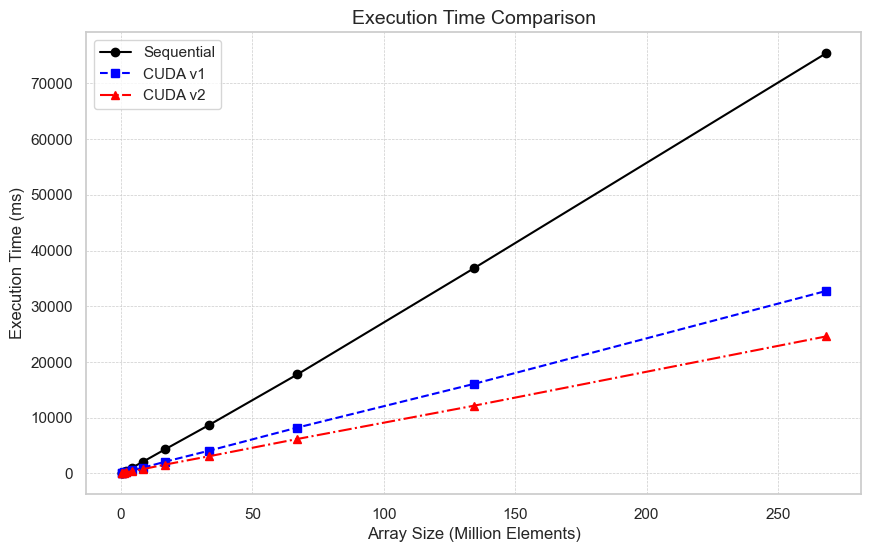
\includegraphics[width=0.6\textwidth]{Images/plot1.png}
  \caption{Execution Time vs Array Size for CUDA}
\end{figure}

\begin{figure}[h]
  \centering
  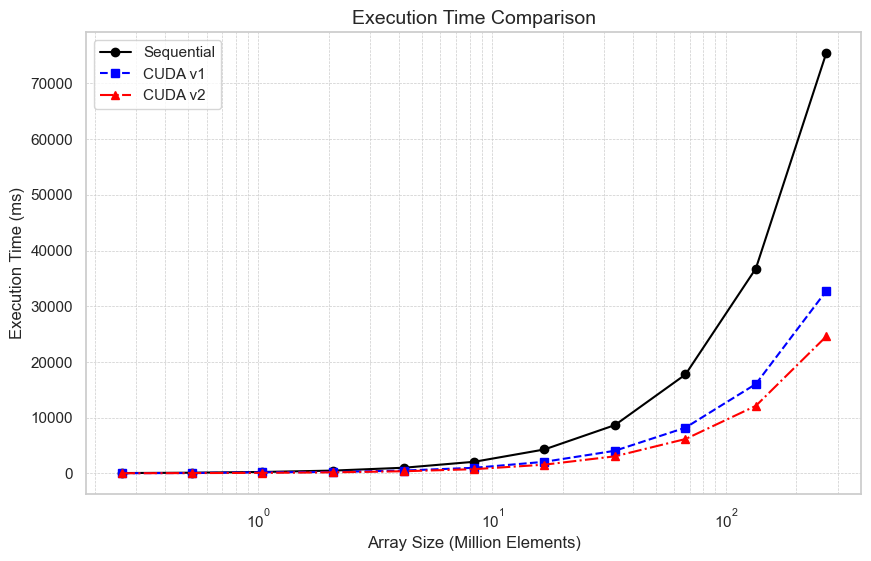
\includegraphics[width=0.6\textwidth]{Images/plot2.png}
  \caption{Execution Time vs Array Size for CUDA, x on log scale}
\end{figure}

\begin{figure}[h]
  \centering
  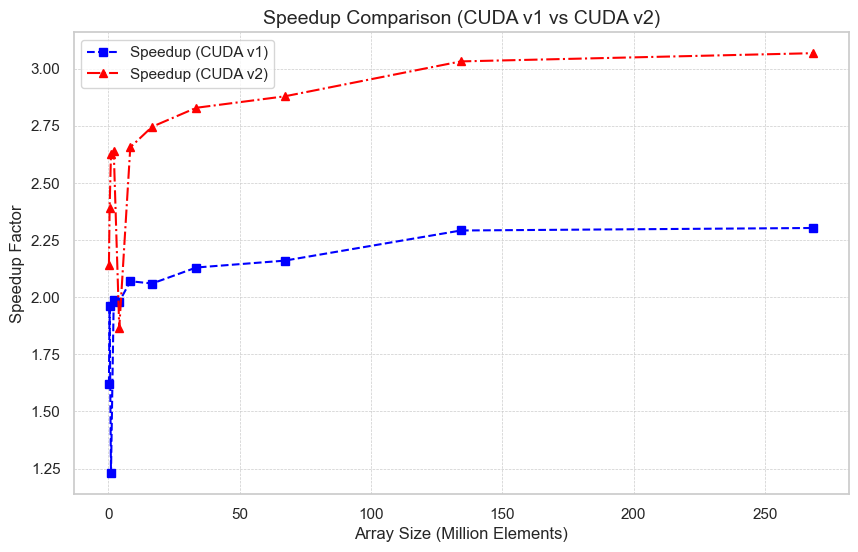
\includegraphics[width=0.6\textwidth]{Images/plot3.png}
  \caption{Speed up vs Array Size for CUDA}
\end{figure}

\begin{figure}[h]
  \centering
  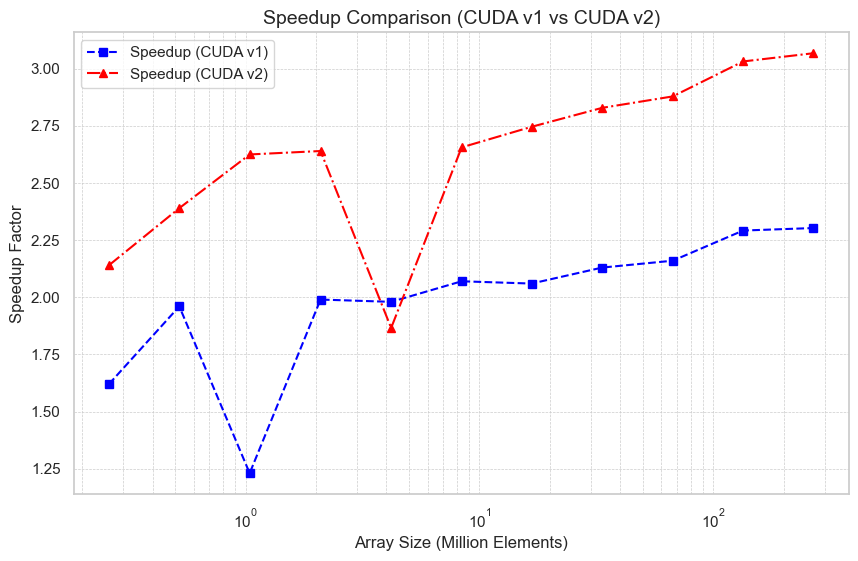
\includegraphics[width=0.6\textwidth]{Images/plot4.png}
  \caption{Speed up vs Array Size for CUDA, x on log scale}
\end{figure}

\begin{figure}[h]
  \centering
  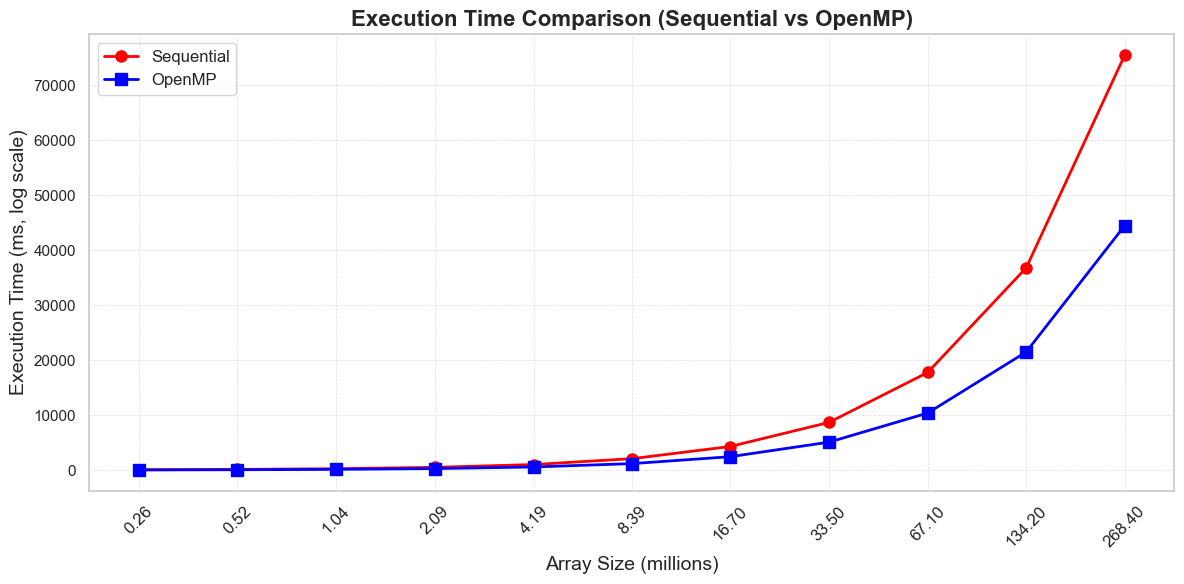
\includegraphics[width=0.6\textwidth]{Images/plot5_xlog.png}
  \caption{Execution Time vs Array Size for Open MP, x on log scale}
\end{figure}

\begin{figure}[h]
  \centering
  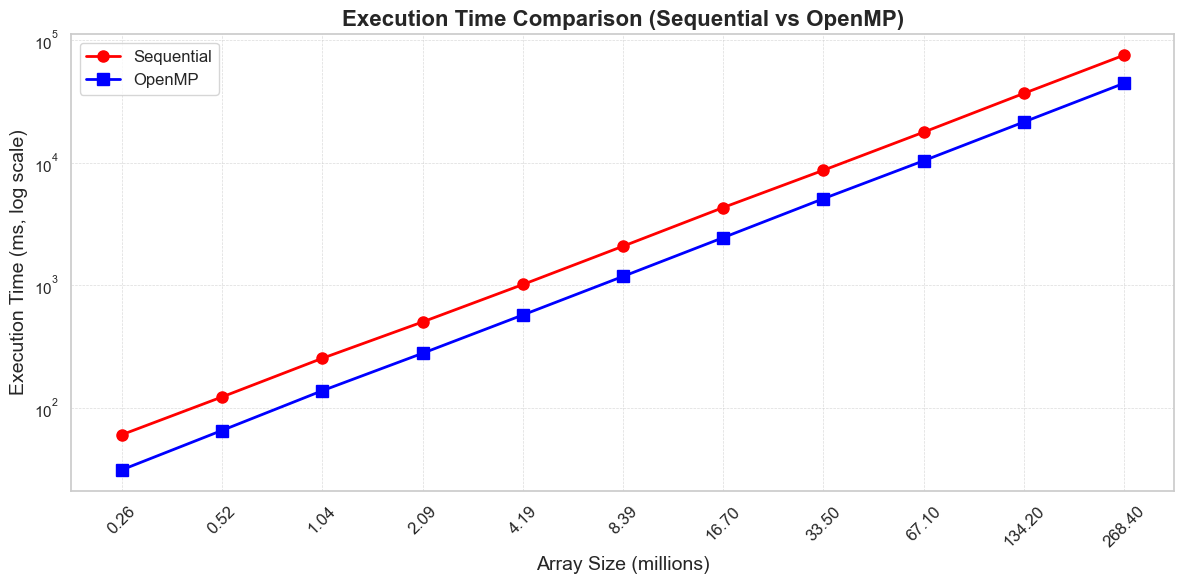
\includegraphics[width=0.6\textwidth]{Images/plot5_xylog.png}
  \caption{Execution Time vs Array Size for Open MP, x and y on log scale}
\end{figure}

\begin{figure}[h]
  \centering
  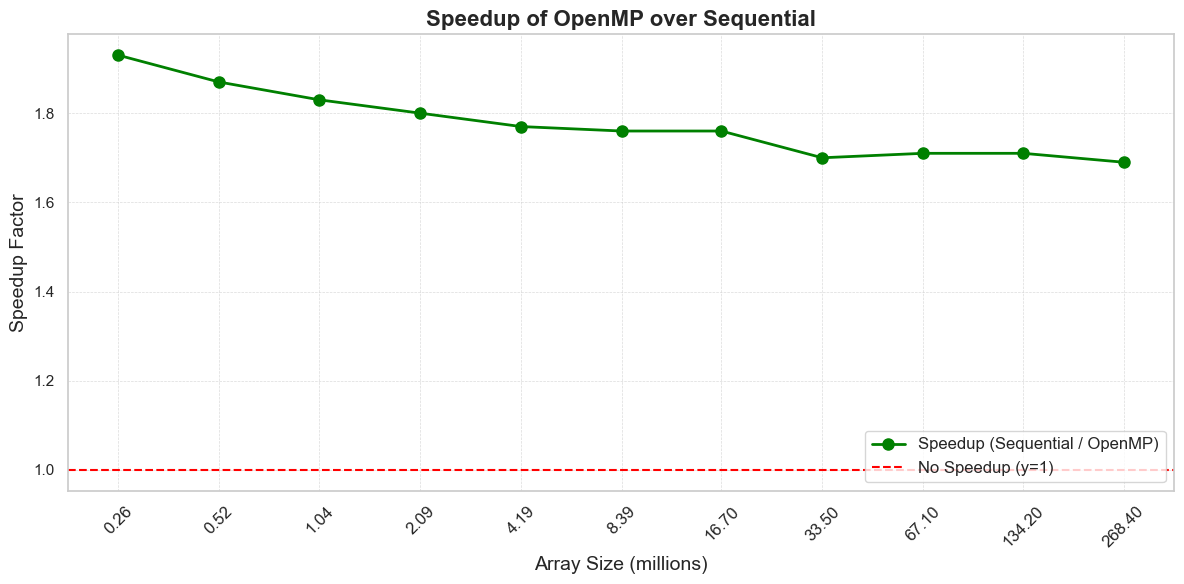
\includegraphics[width=0.6\textwidth]{Images/speedupOpenMP.png}
  \caption{Speed up vs Array Size for Open MP}
\end{figure}


\newpage 

\begin{figure}[h]
  \centering
  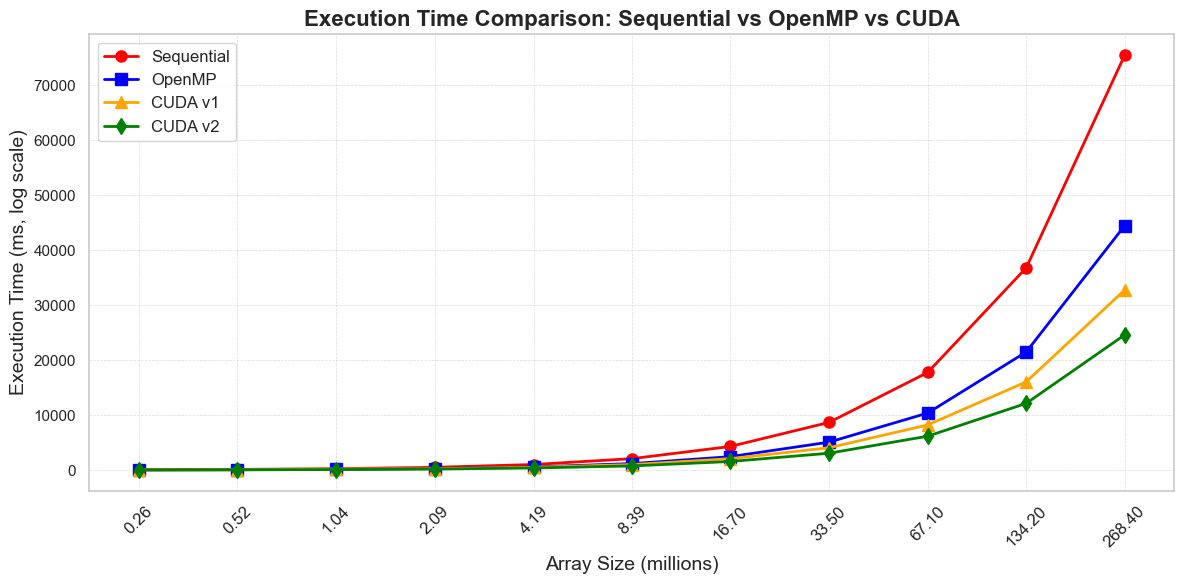
\includegraphics[width=0.6\textwidth]{Images/compare1.png}
  \caption{Comparison on Execution Times}
\end{figure}

\begin{figure}
  \centering
  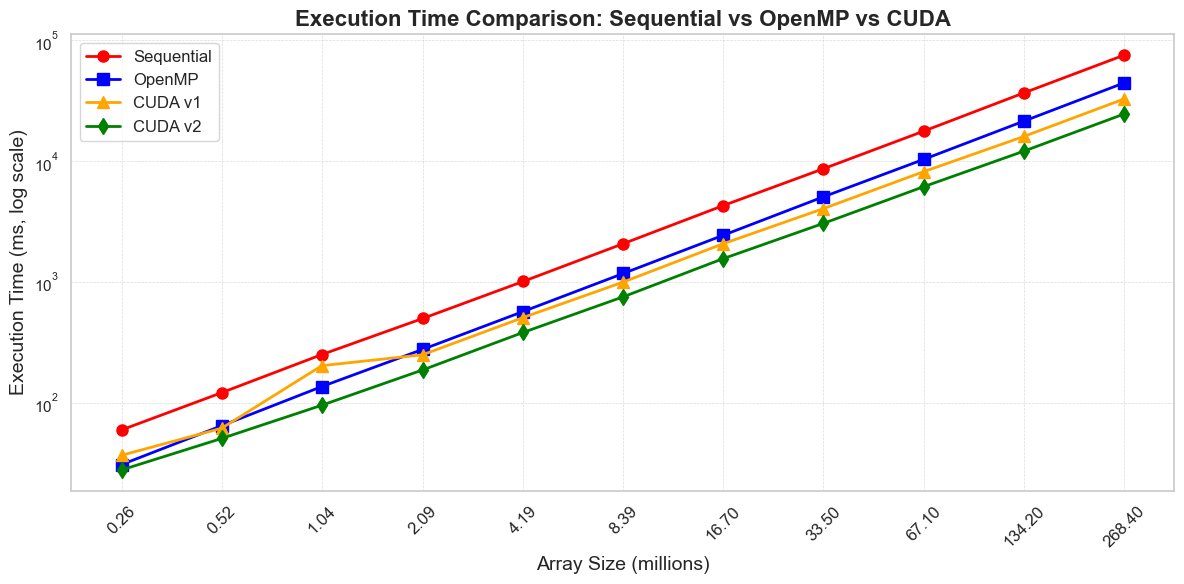
\includegraphics[width=0.6\textwidth]{Images/compare2.png}
  \caption{Comparison on Speedup - x,y on log scale}
\end{figure}

\begin{figure}[h]
  \centering
  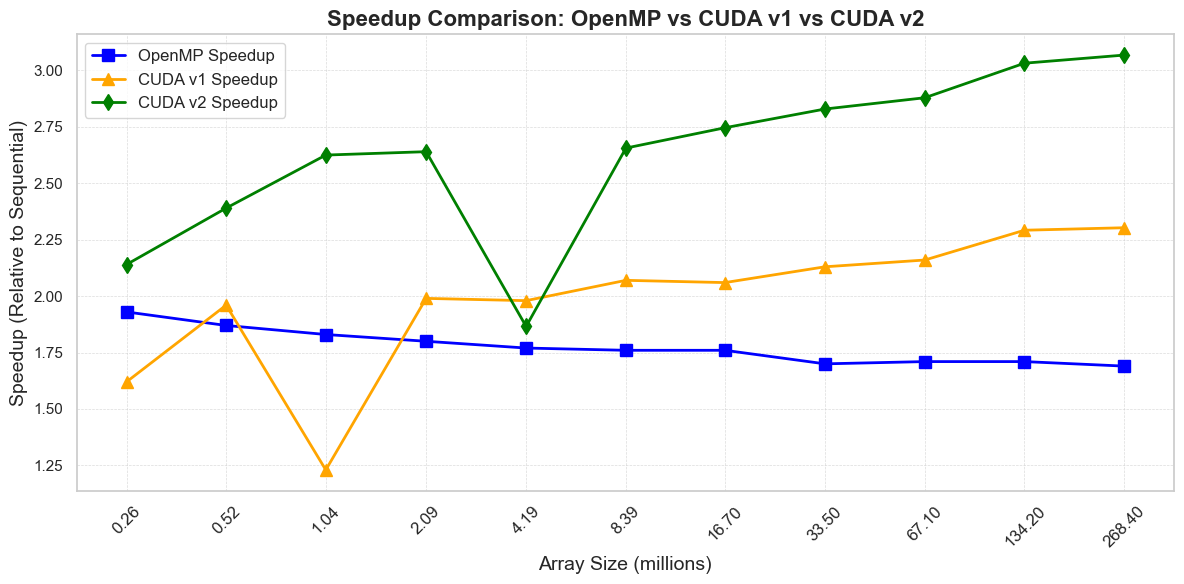
\includegraphics[width=0.6\textwidth]{Images/compare3.png}
  \caption{Comparison on Speedup}
\end{figure}

\newpage

\subsection{CUDA Kernel Profiling Results}

Profiling was conducted using \texttt{nvprof} to analyze the execution performance of the CUDA kernel. The results are summarized as follows:

\subsubsection{GPU Activities}
The majority of GPU execution time was spent in the \texttt{ParallelMergeKernel} function:
\begin{itemize}
    \item \textbf{ParallelMergeKernel:} 99.30\% of total GPU time, with an average execution time of 140.56 ms per call.
    \item \textbf{Memory Transfers:}
    \begin{itemize}
        \item \texttt{[CUDA memcpy HtoD]}: 0.36\% of total GPU time, averaging 5.576 ms per call.
        \item \texttt{[CUDA memcpy DtoH]}: 0.34\% of total GPU time, averaging 5.289 ms per call.
    \end{itemize}
\end{itemize}

\subsubsection{CUDA API Calls}
The CUDA API calls also reflect the kernel execution behavior:
\begin{itemize}
    \item \textbf{\texttt{cudaDeviceSynchronize()}} accounted for 98.50\% of total API execution time, with an average duration of 64.42 ms per call.
    \item \textbf{\texttt{cudaMalloc()}} took 0.78\% of API execution time, averaging 6.13 ms per call.
    \item \textbf{\texttt{cudaMemcpy()}} accounted for 0.70\%, with an average duration of 5.48 ms per call.
\end{itemize}

\subsubsection{Observations and Optimization Potential}
\begin{itemize}
    \item The \texttt{ParallelMergeKernel} function dominates execution time, suggesting that further optimization (such as improved memory access patterns or parallel workload balancing) may enhance performance.
    \item Memory transfers between host and device account for a small but non-negligible portion of execution time. Strategies like memory coalescing and asynchronous transfers could help reduce this overhead.
    \item Frequent calls to \texttt{cudaDeviceSynchronize()} indicate possible inefficiencies, as synchronization stalls execution until all GPU operations are complete.
\end{itemize}


\end{document}
